% Lecture Template for ENGR1120-800 Tristan Hill - Spring 2020
% Dynamics Modeling and Controls
% Chapter 5 - Loops

% I am finally converting my stuff to BEAMER

% Document settings

%\documentclass{beamer}                  % for presentation ?
\documentclass[handout]{beamer}  % for handout ?
\usepackage{beamerthemesplit}
\usepackage{amsmath}
\usepackage{listings}
\usepackage{multicol}
\usepackage{framed}

\beamertemplateballitem

\definecolor{TTUpurple}{rgb}{0.3098, 0.1607, 0.5176} % TTU Purple (primary)
\definecolor{TTUgold}{rgb}{1.0000, 0.8666, 0.0000} % TTU Gold (primary)

\setbeamercolor{palette primary}{bg=TTUpurple,fg=TTUgold}
\setbeamercolor{palette secondary}{bg=black,fg=TTUgold}
\setbeamercolor{palette tertiary}{bg=black,fg=TTUpurple}
\setbeamercolor{palette quaternary}{bg=TTUgold,fg=black}
\setbeamercolor{structure}{fg=TTUpurple} % itemize, enumerate, etc
\setbeamercolor{section in toc}{fg=TTUpurple} % TOC sections

%\usefonttheme{professionalfonts}
\definecolor{mygray}{rgb}{.6, .6, .6}

% [153,50,204] - dark orchid
\definecolor{mypurple}{rgb}{0.6,0.1961,0.8}
%[139,69,19] - saddle brown
\definecolor{mybrown}{rgb}{0.5451,0.2706,0.0745}
\definecolor{mygreen}{rgb}{0,.4,0}
\definecolor{mygray}{rgb}{.6, .6, .6}
\definecolor{mypurple}{rgb}{0.6,0.1961,0.8}
\definecolor{mybrown}{rgb}{0.5451,0.2706,0.0745}
\definecolor{mygreen}{rgb}{0, .39, 0}

\newcommand{\R}{\color{red}}
\newcommand{\B}{\color{blue}}
\newcommand{\BR}{\color{mybrown}}
\newcommand{\K}{\color{black}}
\newcommand{\G}{\color{mygreen}}
\newcommand{\PR}{\color{mypurple}}


\newcommand{\CNUM}{5\hspace{2mm}} % Chapter Number 
\newcommand{\LNUM}{1\hspace{2mm}} % Lecture Number 

\newcommand{\vspcc}{\vspace{6mm}\\ } 
\newcommand{\vspc}{\vspace{2mm}\\ } 
\newcommand{\hspc}{\hspace{5mm} } 

\newcommand{\Lagr}{\mathcal{L}} % lagrangian

\newcommand{\secondtitle}{Using Loop Statements}% second line of the title of this presentation , aka the topic of this lecture

\title{Chapter \CNUM - Lecture \LNUM}
\author{ENGR1120 - 800 - Honors Programming for Engineers} % original formatting from Mike Renfro, September 21, 2004

\date{April 14, 2020}

\begin{document}

\lstset{language=MATLAB,basicstyle=\ttfamily\large,showstringspaces=false}

% Title page1 
\frame{\titlepage \center\textbf{\secondtitle}\vspcc}


% Section 0: Outline
\frame{

\large \textbf{Lecture \LNUM - \secondtitle} \vspc

 \begin{itemize}

	
	\item What is Looping? \vspcc  % Section 1

	\item Types of Loops \vspcc % Section 2

	\item MATLAB Examples \vspcc % Section 3


\end{itemize}

}


%Section 1: What is What is Looping? 
\section{What is Looping?}

\subsection{Repeated Code}
\frame{
\frametitle{Repeated Code}

	
	\large 

You may have you noticed in your programs that there was a lot of \PR Repeated Code \K? Is this OK?\vspc

	\begin{itemize}
		\item 
		\item \vspace{3mm}
	\end{itemize}
	\vspace{3mm}

What can we do about it?  
            			
Introduce a new \color{blue}Control Structure \color{black} ... 
		
}
\subsection{A New Control Structure}
\frame{
\frametitle{A New Control Structure}
	

A loop is a fundamental {\bf control structure} in sequential programming in which one or more commands is executed in repetition controlled by a logical statement or counter. - TH  
\vspace{5mm}\\
... In computer programming, a loop is a sequence of instructions that is repeated until a certain condition is reached.  - Web

	\begin{itemize}
		\item 
		\item \vspace{3mm}
	\end{itemize}
	\vspace{3mm}

}

\subsection{Why use Loops? }
\frame{
\frametitle{Why use Loops? }


         \Large Why are loops useful in computer programming? \vspc
	\large
	\begin{itemize}
		\item Reduce problems associated with {it repeated code} \vspc
		\item \vspace{3mm}
		\item \vspace{3mm}
	\end{itemize}

}

%Section 2: Types of Loops
\section{Types of Loops}

\subsection{Many Different Types}
\frame{
\frametitle{Many Different Types}

\large There are many different types of loops in computer programming. This is not an inclusive list.\vspc
\begin{itemize}

	\item \B WHILE \K loops
	\item \B FOR \K loops
	\item {\it nested} loops
	\item DO... WHILE loops
\end{itemize}

\large Loops can be characterized as {\it entry-controlled} or {\it exit-controlled} loops.

}

\subsection{The WHILE Loop}
\frame{
\frametitle{The WHILE Loop}

 The WHILE Loop is  the simplest loop in computer programming.\vspc
\begin{itemize}

	\item {\bf block of code} is repeated as long as \textbf{\PR condition} \K is\textbf{ \G true } \K \vspc
	\item {\it entry-controlled} loop structure \vspc
	\item \vspace{3mm}
	\item  \vspace{3mm}

\end{itemize}

}

\subsection{Structure of a WHILE Loop}
\frame[containsverbatim]{
\frametitle{Structure of a WHILE Loop}

%It is useful to visualize the structure in a {\bf program flowchart} \vspcc
%%\begin{multicols}{2}
%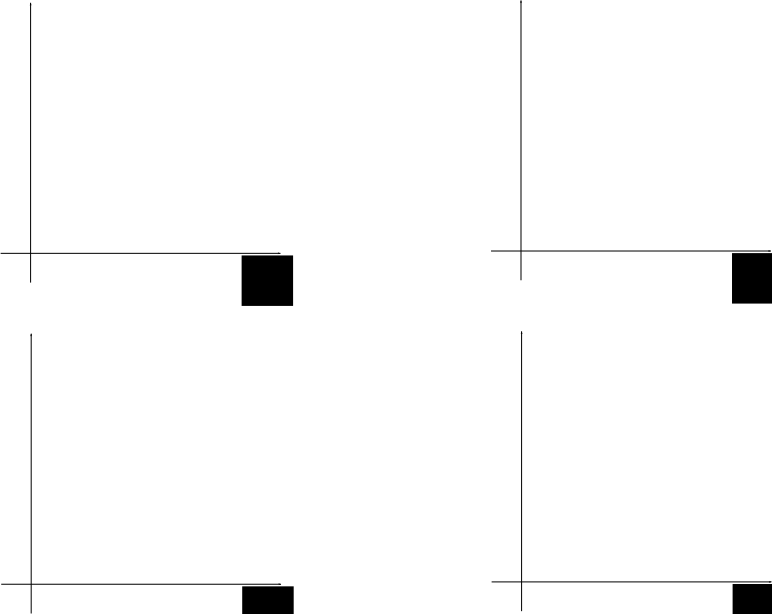
\includegraphics[scale=0.25]{lecture1_fig1.png}\\	
%
\begin{framed}
\begin{lstlisting}
i=1; %Initialize the Counter

while(i<10)

	% Do Stuff Here

	i=i+1; % Increment the Counter

end	
\end{lstlisting}
\end{framed}
%
%%\end{multicols}
}


%Section 3: MATLAB Examples


% references is not a section for now, for looks and it would be a waste of space
\frame{

\frametitle{References}

\begin{itemize}
	\item Your MATLAB textbook - Chapter 5 - Looping Statements
\end{itemize}

}
\end{document}









 